\documentclass[]{article}
\usepackage{xcolor}
\usepackage{listings}
\usepackage{showexpl}
\usepackage[bahasai]{babel}
\usepackage{graphicx}
\lstset{language=C++,
	% numbers=left,
	%	stepnumber=1,
	numberstyle=\ttfamily,
	basicstyle=\ttfamily,
	keywordstyle=\color{blue}\ttfamily,
	stringstyle=\color{red}\ttfamily,
	commentstyle=\color{gray}\ttfamily,
	morecomment=[l][\color{magenta}]{\#}
}


%opening
\title{Tugas 3: Implementasi Stack}
\author{Akhmad Thoriq Afif NRP 5024201028}

\begin{document}
\maketitle
\section{Listing Program}
Di bawah ini merupakan program implementasi struktur data stack menggunakan bahasa C++
\lstinputlisting[label={kodingan},caption={Implementasi Struktur Stack}, language={C++}]{usinglinked.cpp}
\pagebreak
\subsection*{OUTPUT PROGRAM:}
\begin{figure}[htp]
    \centering
    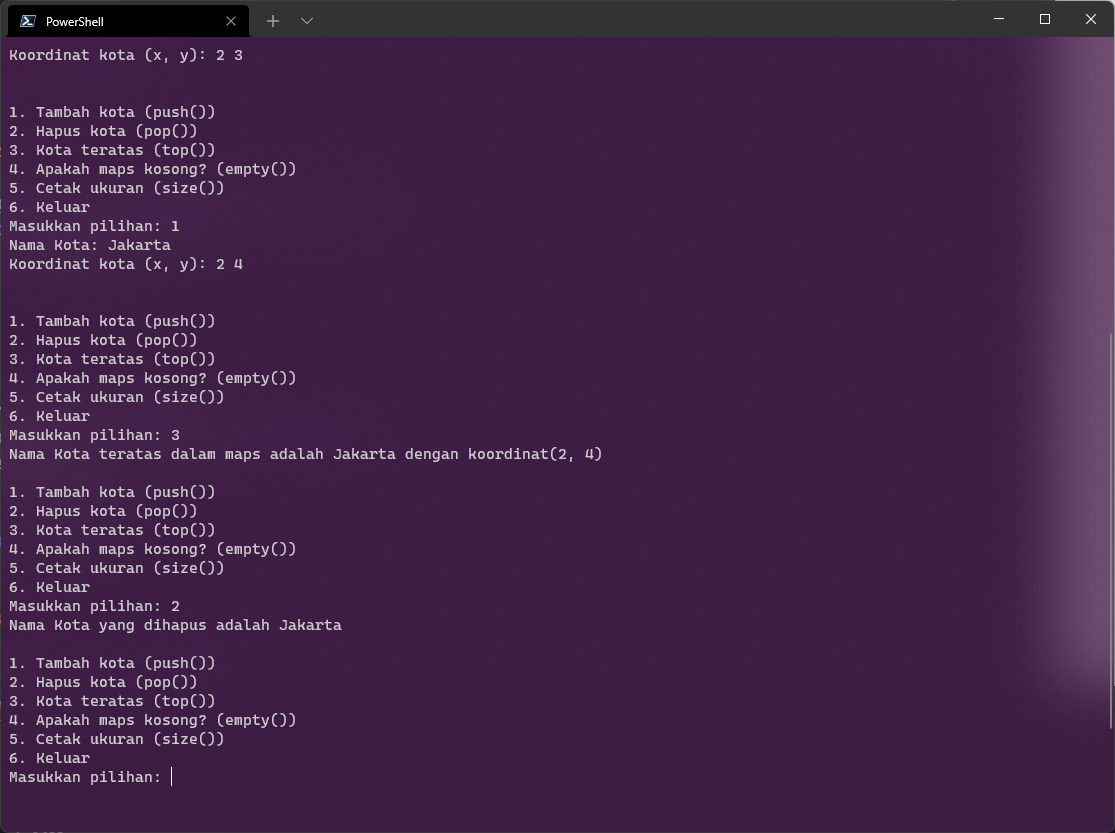
\includegraphics[width=12cm]{output.png}
    \caption{Output Program}
    \label{fig:galaxy}
\end{figure}
\pagebreak
\section{Penjelasan Program}
\subsection{Desain struktur data}
\par
Pada desain struktur data ini terdapat dua class yaitu Node dan Stack. 
Class Node berisikan variabel data dan previous yang berfungsi untuk menyimpan
objek dan Node yang terletak di bawahnya dalam bentuk pointer. 
Class Node ini berada didalam Class Stack atau bisa disebut sebagai
Nested Class. Tujuannya agar class Node tidak dapat diakses dari luar
Class Stack. Untuk Class Stack berisikan fungsi fungsi dasar untuk
melakukan perubahan pada stack. Class inilah yang nantinya akan digunakan untuk menyimpan suatu objek.
Gambar di bawah ini merupakan visualiasasi dari kedua class tersebut.
\begin{figure}[htp]
    \centering
    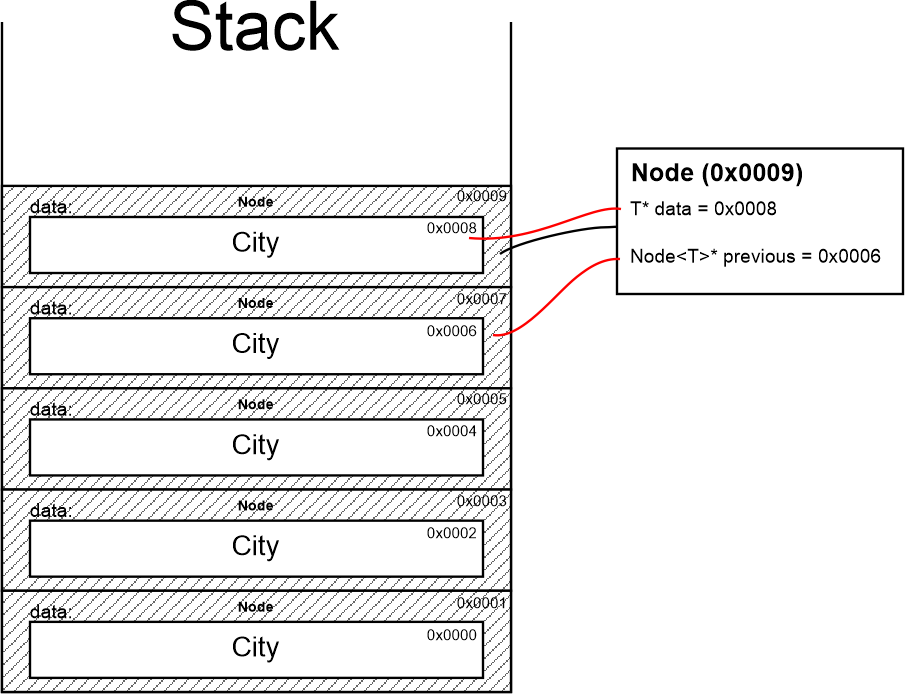
\includegraphics[width=5cm]{visualisasi.png}
    \caption{Desain struktur data Stack}
    \label{fig:galaxy}
\end{figure}
\subsection{Fungsi push()}
\lstinputlisting[label={maxvalue},caption={Fungsi untuk menambah kota}, language={C++}, firstline=34, lastline=40]{usinglinked.cpp}
\par
Fungsi ini berfungsi untuk memasukkan objek kedalam stack. Fungsi ini membutuhkan satu parameter yaitu objek yang
akan dimasukkan kedalam stack. Cara kerja dari fungsi ini adalah pertama objek yang akan dimasukkan di-contruct ulang
menggunakan new, yang mana dengan menggunakan new ini akan membuat objek tersimpan di dalam heap dan mereturn pointer dari objek tersebut. 
Pointer tersebut akan dijadikan sebagai parameter dalam pembuatan Node. Node ini disimpan kedalam variabel tempNode. Langkah selanjutnya,
previous yang terdapat dalam tempNode diisi dengan pointer mCurrentNode. Sedangkan, mCurrentNode diisi dengan pointer tempNode. Terakhir,
dilakukan penambahan mSize dengan 1.
\subsection{Fungsi pop()}
\lstinputlisting[label={maxvalue},caption={Fungsi untuk menghapus kota}, language={C++}, firstline=42, lastline=50]{usinglinked.cpp}
\par
Fungsi ini berfungsi untuk menghapus objek teratas dari stack dan mengembalikan objek yang telah terhapus. Fungsi ini tidak membutuhkan parameter. Cara kerja dari fungsi ini adalah
pertama, data yang terdapat dalam mCurrentNode disimpan kedalam variabel temp. Selanjutnya, Node previous yang terdapat dalam mCurrentNode disimpan ke dalam tempNode.
Kemudian, dilakukan pemanggilan destructor objek yang tersimpan dalam mCurrentNode menggunakan delete. Hal ini dilakukan agar mengurangi penggunaan memory. Setelah dihapus, mCurrentNode diisi dengan tempNode.
Sebelum melakukan return, mSize di-decrement dengan 1. Karena scope dari variabel temp hanya bersifat lokal, ketika fungsi selesai dijalankan objek temp ini akan otomatis terhapus sehingga jika ingin diakses
maka akan terjadi error Memory Access Violation. Maka dari itu digunakan std::move sebelum melakukan return.
\end{document}
